\documentclass[aspectratio=1610]{beamer}
\usepackage[utf8]{inputenc}

% Load color with all needed options BEFORE other packages that might use it
\PassOptionsToPackage{table}{xcolor}
\usepackage{xcolor}

\usepackage{graphicx}
\usepackage{MnSymbol}
\usepackage{stmaryrd}
\usepackage{colortbl}
\usepackage{caption}
\usepackage{comment}
\usepackage{pdfpages}
\usepackage{listings}
\usepackage{booktabs}
\usepackage{soul}
\usepackage[normalem]{ulem}

\usepackage{tikz}
\usepackage{rotating}
\usepackage{amsmath}
\usetikzlibrary{arrows.meta} 

\usepackage{tcolorbox}
\usepackage{lipsum}
\usepackage{pgf}
\usepackage{etex}
\usepackage{tikz,pgfplots}
\usepackage{ragged2e}
\usepackage{subfig}
\usepackage{beamerthemesplit}
\usepackage{mathtools}

\usetheme{metropolis}

\usepackage[style=authoryear,sorting=nyt]{biblatex}
% \addbibresource{lit.bib}

\newenvironment{wideitemize}{\begin{itemize}\addtolength{\itemsep}{10pt}}{\end{itemize}}
\usepackage{appendixnumberbeamer} % For backup slides

% Define a new theorem-like environment for propositions
\newtheorem{proposition}{Proposition}

% \newenvironment{wideitemize}{\itemize\addtolength{\itemsep}{10pt}}{\enditemize}

\newcommand{\sym}[1]{\ifmmode ^{\text{#1}} \else \textsuperscript{#1}\fi}

\definecolor{myblue}{HTML}{23373B}
\definecolor{myorange}{HTML}{EB811B}
\definecolor{mygreen}{HTML}{14B03E}


\setbeamertemplate{itemize subsubsubitem}{$\triangleright$}   % First level: Bullet
\setbeamertemplate{itemize subitem}{$-$}  % Second level: Diamond
\setbeamertemplate{itemize subsubitem}{$\circ$}  % Third level: Triangle

%%%%%%%%%%%%%%%%%%%%%%%%%%%%%%%%%%%%%%%%%%%%%%%%%
\setbeamertemplate{footline}{
  \leavevmode%
  \hbox{%
    \begin{beamercolorbox}[wd=.4\paperwidth,ht=2.25ex,dp=1ex,center]{author in head/foot}%
      \usebeamerfont{author in head/foot}\insertshortauthor
    \end{beamercolorbox}%
    \begin{beamercolorbox}[wd=.6\paperwidth,ht=2.25ex,dp=1ex,center]{title in head/foot}%
      \usebeamerfont{title in head/foot}\insertshorttitle\hspace*{3em}
      \insertframenumber{} / \inserttotalframenumber\hspace*{1ex}
    \end{beamercolorbox}%
 }%
  \vskip0pt%
}
\setbeamertemplate{navigation symbols}{}

\definecolor{mybgcolor}{RGB}{255, 255, 255}
\setbeamercolor{background canvas}{bg=mybgcolor}

\lstset{frame=tb,
 language=Java,
 aboveskip=2mm,
 belowskip=2mm,
 showstringspaces=false,
 columns=flexible,
 basicstyle={\small\ttfamily},
 numbers=none,
 numberstyle=\tiny\color{gray},
 keywordstyle=\color{blue},
 commentstyle=\color{dkgreen},
 stringstyle=\color{mauve},
 breaklines=true,
 breakatwhitespace=true,
 tabsize=2
}

\title{Remote Work and the Wage Premium}
\author{Mitchell Valdes-Bobes and Anna Lukianova}
\date{\today}

\begin{document}

% Title slide
{
  \setbeamertemplate{footline}{}
  \begin{frame}
    \titlepage
  \end{frame}
}
\addtocounter{framenumber}{-1}

% Slide 1: Research Question and Motivation
\begin{frame}{Research Question}
\textbf{Research Question:} How does the feasibility of remote work influence the wage premiums of remote workers?
\vspace{1cm}
% %\pause

\textbf{Agenda for \sout{Today}}
\begin{itemize}  
    \item \textbf{Occupation Remote Index:} New a measure of remote work feasibility.
    \begin{itemize}
        \item[\textbf{\textcolor{red}{Mistake}}] This took too much time in the presentation and was not the main focus. 
    \end{itemize}
    \item \textbf{Theoretical Model:} Remote work and worker-firm matching dynamics.
    \begin{itemize}
        \item[\textbf{\textcolor{blue}{Well recieved}}] The assumptions and the model were well received. Would like to have more time to discuss the model. I got the comment that presenting the model first would have been better since it would have disciplined the audience on how to think about the situation.
    \end{itemize}
    \item \textbf{Model Calibration \& Preliminary Results:} Key findings and next steps. 
    \begin{itemize}
        \item[\textbf{Feedback}] I did not get to spend time on this part of the presentation. The calibration is still in progress and would like to get more feedback.
    \end{itemize}
    
\end{itemize}  

\end{frame}  


\begin{frame}{Related Literature}
    \begin{itemize}
        \item[I.] \textbf{Teleworkability Measurement} 
        \begin{itemize}
            \item \textbf{Dingel, Neiman (2020), Mongey, Pilossoph, Weinberg (2021)} Construct teleworkability indices using occupation tasks and requirements based on ad hoc feature selection.
            \begin{itemize}
                \item \textbf{Contribution} Use machine learning on a high-dimensional feature set, rather than relying on manual selection.
            \end{itemize}
        \end{itemize}
        \vspace{0.3cm}
        
        % %\pause
        \item[II.] \textbf{Remote Work and Compensation}
        \begin{itemize}
            \item \textbf{Pabilonia, Vernon (2023), Cullen, Pakzad-Hurson, Perez-Truglia (2024), Barrero, Bloom, Buckman, and Davis (2023)} Workers value remote work document wage premiums associated with remote work.
            \begin{itemize}
                \item \textbf{Contribution} Link wage premiums to occupation teleworkability.
            \end{itemize}
        \end{itemize}
        % %\pause

        \vspace{0.3cm}
        \item[III.] \textbf{Amenity Provision and Hedonic Wages}
        \begin{itemize}
            \item \textbf{Morchio, Moser (2024), Hwang, Mortensen, Reed (1998)} Model how workers value job amenities and how these preferences affect wages. 
            \begin{itemize}
                \item \textbf{Contribution} Link worker preferences for remote work to job productivity. Allow for heterogeneity in remote work efficiency at the firm and worker level.
            \end{itemize}
        \end{itemize}
    \end{itemize}
\end{frame}




% Slide 2: Empirical Evidence
\section{Empirical Evidence}
% --- Main Presentation Slides ---

\begin{frame}{Data Sources and Sample Characteristics}
    \begin{itemize}
        \item \textbf{American Community Survey, 2013-2022}: individual data.
        \begin{itemize}
            \item Sample civilian wage-employed, respondents between 22 and 70, work more than 30 hours over federal minimum wage.
            \item Remote work defined as not commuting to work \textit{(answered: worked from home)}.
        \end{itemize} %\pause \vspace{0.3cm}
        \item \textbf{ONET}: occupation level data.
        \begin{itemize}
            \item Skills, abilities, work context, and work activities.
        \end{itemize}%\pause \vspace{0.3cm}
        \item \textbf{BLS}: occupation-industry level data.
        \begin{itemize}
            \item Selected occupation feasibility of remote work.
            \item Occupational composition of the workforce. (U.S. and 3-digit industry level).
            \item Labor productivity at the 3-digit industry level.
            \item Occupational Requirements Survey (ORS) establishment-level data that includes teleworkability at the occupation level (incomplete coverage).
        \end{itemize}%\pause \vspace{0.3cm}
        \item \textbf{Other}:
        \begin{itemize}
            \item Business Dynamics Statistics (BDS).
            \item WFH Map, \textbf{Hansen, et. al. (2023)}: Remote job posting.
        \end{itemize}
    \end{itemize}
\end{frame}

\begin{frame}[label=balance]{Remote vs. Non-Remote Worker Characteristics}
\small
\begin{table}[H]
    \centering
    \begin{tabular}{lcccc}
        \hline
        \hline
     & \multicolumn{2}{c}{\textbf{Non-WFH}} & \multicolumn{2}{c}{\textbf{WFH}}\\
    \hline
     & Mean & Sd & Mean & Sd \\
    \hline 
 Share labor force 2013 - 2019 & 97\% & - & 3\% & - \\
 Share labor force 2020 - 2023 & 85\% & - & 15\% & - \\
 Age   & 44.20 & 12.43 & 44.66& 11.88  \\
 Total income  & 67,536.4 & 69,200.87 & 106,556.2 & 97,919.89 \\
 Hourly wage  & 27.95 & 25.81  & 44.20 & 37.59 \\
 Real hourly wage & 26.31 & 24.10 & 39.31 & 33.10\\
 Commuting time  & 26.81 & 23.50 & - & -   \\
 Share of College  & 39\% & - & 66\% & - \\  
 Share of Postgraduate  & 15\% & - & 26\% & - \\
    \hline
    \hline
 Observations  & \multicolumn{2}{c}{9025857} & \multicolumn{2}{c}{751654}\\ 
        \hline
        \hline
    \end{tabular}
    \label{summary_stat}
\end{table}

\end{frame}

\begin{frame}{Teleworkability Index}
    \begin{itemize}
        \item \textbf{Teleworkability Index:} A measure of the extent to which an occupation can be performed remotely. %\pause \vspace{0.3cm}
        \item \textbf{Why?:} Are there inherent occupational characteristics that not only make a job teleworkable but also imply higher wages? %\pause \vspace{0.3cm}
        \item Existing teleworkability indexes are coarse and use inconsistent feature selection.
        \begin{itemize}
            \item \textbf{Dingel and Neiman (2020)} classify occupations as teleworkable or not.
            \item \textbf{Mongey, Pilossoph, Weinberg (2021)} measured occupation feasibility for remote work and physical proximity required.
            \item Both approaches require the researcher to make assumptions about the importance of the features used to classify teleworkability.
        \end{itemize} %\pause \vspace{0.3cm}
        \item \textbf{Need for a New Index:}
            \begin{itemize}
                \item Leverage a high-dimensional, data-driven approach.
                \item Capture nuanced differences in how tasks and requirements enable remote work.
            \end{itemize}
    \end{itemize}
\end{frame}

\begin{frame}{Teleworkability Index}
    \begin{itemize}
        \item \textbf{Need for a New Index:}
            \begin{itemize}
                \item \textbf{\textcolor{red}{Need to highlight why a 0 or 1 classification is not enough. Need to compare the results of the main regressions with the teleworkability index and the 0 or 1 classification. The index is also used in calibration.}}
                \item Leverage a high-dimensional, data-driven approach.
                \item Capture nuanced differences in how tasks and requirements enable remote work.
                \item \textbf{\textcolor{red}{Need to compare the accuracy of the index with the existing classifications.}}
            \end{itemize}
    \end{itemize}
\end{frame}

\begin{frame}[label=empiric_remote_index1]{Occupation Remote Index}
    \begin{itemize}
        \item \textbf{Approach:} Use a mixture of machine learning models to generate a teleworkability index. \hyperlink{appendix_remote_index_details}{\beamergotobutton{details}}%\pause \vspace{0.3cm}
        \begin{itemize}
            \item Classify occupations as teleworkable or not and score their teleworkability.
            \item Identify key contributing occupational features.%\pause \vspace{0.3cm}
            \begin{itemize}
                \item \textbf{Classifier Stage:} Feature importance identifies occupations impossible to telework. (\textit{extensive margin})\hyperlink{appendix_remote_index_performance_feature_importance_classifier}{\beamergotobutton{details}}
                \item \textbf{Regressor Stage:} Feature importance the level of teleworkability. (\textit{intensive margin})\hyperlink{appendix_remote_index_performance_feature_importance_regressor}{\beamergotobutton{details}}
            \end{itemize}
        \end{itemize}%\pause \vspace{0.3cm}
        \item Validate results against labeled occupational data. \vspace{0.3cm}
        \begin{itemize}
            \item Establishment-level data: Percentage of workers that are \textbf{able} to telework at the occupation level.
            \item The coverage is incomplete, we use the provided values and the estimated index to predict the teleworkability of the remaining occupations.
        \end{itemize}
    \end{itemize}
\end{frame}
        
\begin{frame}[label=empiric_remote_index2]{Classifier/Regressor Performance and Data Distribution}
        \begin{columns}
            \column{0.3\textwidth}
            {\small % This makes the font smaller for the left column
                \begin{itemize}\small
                    \item \textbf{Classification:} 
                    \begin{itemize}\footnotesize
                        \item Accuracy = 90.7\%
                        \item F1 =91.9\%
                    \end{itemize}
                    \item \textbf{Regression:}
                    \begin{itemize}\footnotesize
                        \item MSE = 0.1
                        \item Correlation = 0.71
                    \end{itemize}
                \end{itemize}
            }
            \column{0.7\textwidth}
                \begin{figure}
                    \centering
                    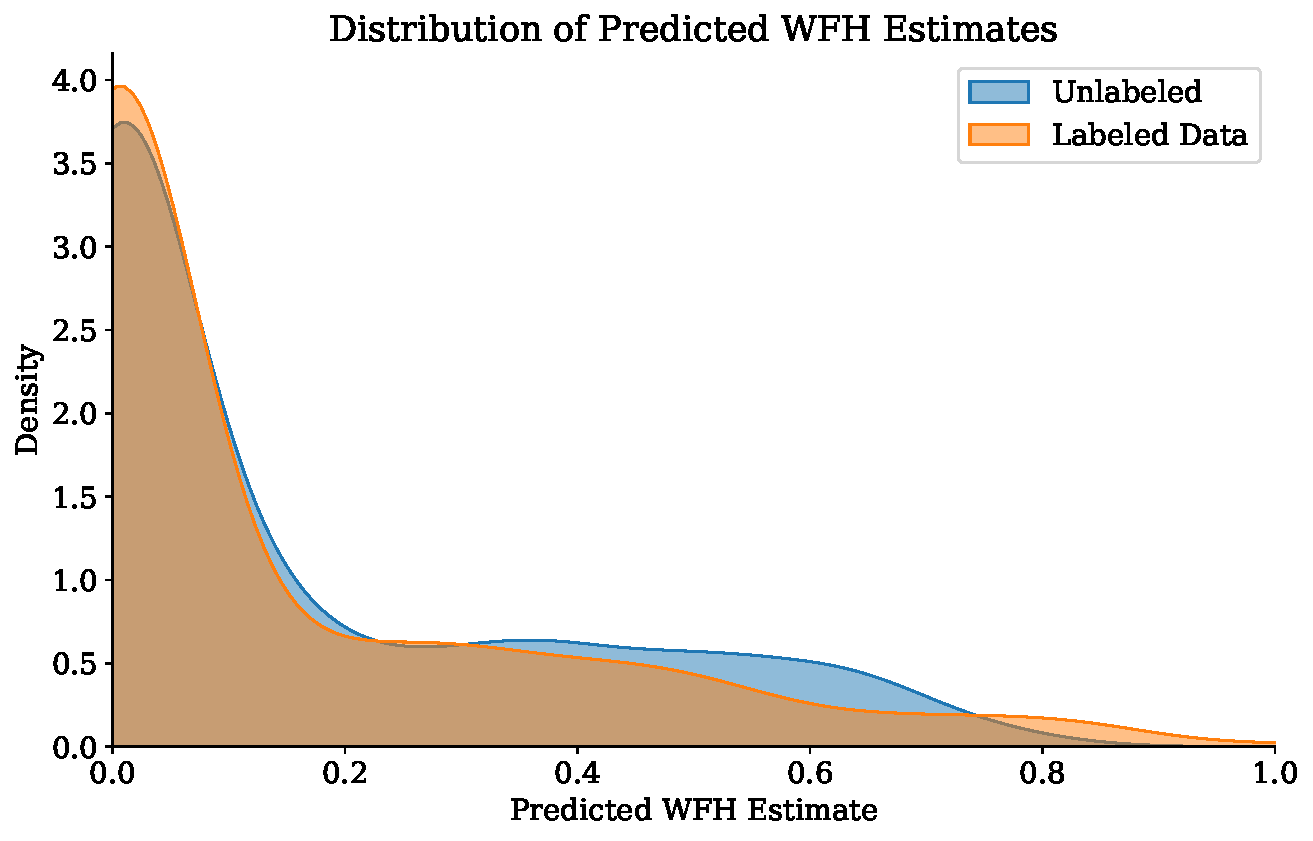
\includegraphics[width=\textwidth]{/Users/mitchv34/Work/WFH/figures/telework_index_estimation/unlabeled_prediction.pdf}
                    \caption{Distribution of Unlabeled vs Labeled Data}
                \end{figure}
        \end{columns}
    \end{frame}
            
    
    

\begin{frame}[label = sfact_1_logwage]{Stylized Fact I: Remote Work Correlates with Higher Wages}
    \begin{table}[htbp]
        \centering
        \footnotesize
        \caption{(log)Wage regressed on Teleworkability index and remote work indicator.}
        \begin{tabular}{l c c c c c >{\columncolor{myorange!20}}c}
        \hline \hline  
                            &\multicolumn{1}{c}{(1)}         &\multicolumn{1}{c}{(2)}         &\multicolumn{1}{c}{(3)}         &\multicolumn{1}{c}{(4)}         &\multicolumn{1}{c}{(5)}         &\multicolumn{1}{c}{(6)}         \\
        \hline
 Teleworkability Index          & 1.009\sym{***}& 0.860\sym{***}& 0.582\sym{***}& 0.551\sym{***}& 0.484\sym{***}& 0.473\sym{***}\\
                            & (0.00111)         & (0.00129)         & (0.00256)         & (0.00256)         & (0.00124)         & (0.00124)         \\
 WFH Indicator              &                     &                     &                     & 0.161\sym{***}&                     & 0.0793\sym{***}\\
                            &                     &                     &                     & (0.000970)         &                     & (0.000909)         \\
        \hline
 FE: Year \& Location            &  $\checkmark$  &  $\checkmark$  &  $\checkmark$  &  $\checkmark$  & $\checkmark$  &   $\checkmark$  \\
 FE: Industry                    &                &  $\checkmark$  &               &  $\checkmark$  &  $\checkmark$  &  $\checkmark$  \\
 AgeCat  $\times$ Educ                &                &               &               &               &  $\checkmark$    &  $\checkmark$  \\
        \hline
 N                   & 9708029         & 9708029         & 9708029         & 9708029         & 9708028         & 9708028         \\
        $R^2$                  & 0.198         & 0.279         & 0.334         & 0.338         & 0.420         & 0.421         \\
        \hline\hline
        \multicolumn{7}{l}{\footnotesize Worker level data. All regressions include demographic controls: age, race, education, others.}\\
        \multicolumn{7}{l}{\footnotesize Standard errors in parentheses: \sym{*} \(p<0.1\), \sym{**} \(p<0.05\), \sym{***} \(p<0.001\).}\\
    \end{tabular}
    \end{table}
    \hyperlink{sfact_1_wage}{\beamerskipbutton{Wage regression}}
\end{frame}

\begin{frame}[label = sfact_2_logwage]{Stylized Fact II: Within Occupations Remote Workers Earn More}

\begin{table}[htbp]
    \centering
    \footnotesize
    \caption{(log)Wage regressed on remote work indicator and controls. }
    \begin{tabular}{l c c c c >{\columncolor{myorange!20}}c}
    \hline\hline  
                    & \multicolumn{1}{c}{(1)}         & \multicolumn{1}{c}{(2)}         & \multicolumn{1}{c}{(3)}         & \multicolumn{1}{c}{(4)}         & \multicolumn{1}{c}{(5)}         \\
\hline
WFH Indicator              & 0.347\sym{***} & 0.216\sym{***} & 0.146\sym{***} & 0.130\sym{***} & 0.0880\sym{***} \\
                    & (0.00108)         & (0.00105)         & (0.000946)         & (0.000942)         & (0.000870)         \\
\hline
FE: Year \& Location            &  $\checkmark$  &  $\checkmark$  &  $\checkmark$  &  $\checkmark$  &  $\checkmark$  \\
FE: Industry                    &                &  $\checkmark$  &               &  $\checkmark$  &  $\checkmark$  \\
FE: Occupation                  &                &               &  $\checkmark$  &  $\checkmark$  &  $\checkmark$  \\
FE: Class of Worker             &                &               &               &  $\checkmark$  &  $\checkmark$  \\
AgeCat  $\times$ Educ                &                &               &               &               &  $\checkmark$  \\
\hline
N                   & 9712293         & 9712293         & 9712293         & 9712293         & 9712292         \\
$R^2$               & 0.0955         & 0.227         & 0.383         & 0.408         & 0.485         \\
\hline\hline
\multicolumn{6}{l}{\footnotesize Worker level data. All regressions include demographic controls: age, race, education, others.}\\
\multicolumn{6}{l}{\footnotesize Standard errors in parentheses: \sym{*} \(p<0.1\), \sym{**} \(p<0.05\), \sym{***} \(p<0.001\).}\\
    \end{tabular}
\end{table}
\hyperlink{sfact_2_wage}{\beamerskipbutton{Wage regression}}
\end{frame}


\begin{frame}[label=wfhyears_main]{Stylized Fact III: WFH Wage Premium is Increasing}
\begin{figure}[H]
    \centering
    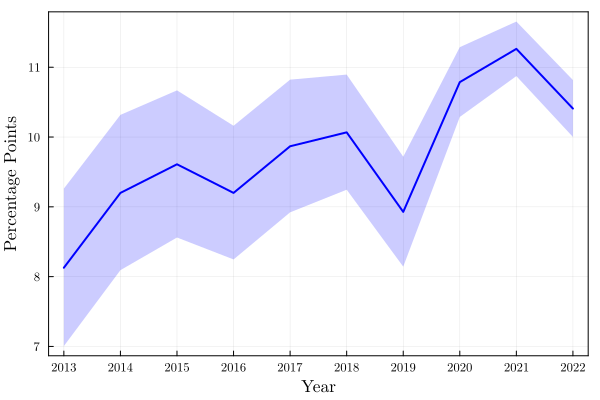
\includegraphics[width=.7\linewidth]{/Users/mitchv34/Work/WFH/figures/wfh_over_years_total_interpretable_no_title.png}
    \label{wfh_over_time}
    \hyperlink{wfhyears_appendix}{\beamerskipbutton{Regression}}
    % \caption*{\footnotesize WFH premium obtained }
\end{figure}
\end{frame}

\begin{frame}{Other Questions and Comments}
    \begin{itemize}
        \item[]\textbf{Question:} How is the transportation question asked in the ACS?
        \begin{itemize}
            \item[] \textcolor{myorange}{Answer:} How did this person usually get to work LAST WEEK?
            \item[] \textcolor{mygreen}{Alternatives:} Incorporate alternative data sources (American Time Use Survey, The Survey of Working Arrangements and Attitudes (SWAA))  
        \end{itemize}
        \item[] \textbf{Question:} How to deal with unobserved heterogeneity? \textit{Rasmus:} Workers who work remotely are vastly different from those who do not. \textit{Carter:} the story might be smart people are able to WFH. (Then the estimate on teleworkability will be upward biased)
        \begin{itemize}
            \item[] \textcolor{myorange}{Answer:} Need to compare workers with similar skills and characteristics that differ in remote work.
            \item[] \textcolor{myorange}{Answer:} Include skill requirements (cognitive, physical and social) of the occupation in the regression. Control for occupation groups (SOC codes or the ONET related occupation measure).
        \end{itemize}
        \item[] 
    \end{itemize}
\end{frame}

% Slide 3: Model
\section{Model}
% --- Slide: Model Overview ---
\begin{frame}{Model Overview}
  \begin{itemize}
    \item Directed search model in the spirit of \textbf{Menzio and Shi (2010)}.%\pause \vspace{0.3cm}
    \item Sources of heterogeneity:\vspace{0.3cm}
    \begin{itemize} 
      \item \textbf{Firms}: Different remote-work efficiencies.
      \item \textbf{Workers}: Different skill levels.
    \end{itemize}%\pause \vspace{0.3cm}
    \item \textbf{Key Mechanisms}:\vspace{0.3cm}
    \begin{itemize}
        \item  Workers value the flexibility provided by remote work arrangements.
        \item High skilled workers are more productive and better suited for remote work.
        \item Firms treat remote and on-site work as substitutable.
    \end{itemize}
  \end{itemize}
\end{frame}

% --- Slide: Workers ---
\begin{frame}{Workers}
  \begin{itemize}
    \item Characterized by their productivity. \vspace{0.3cm}%\pause
    \item Incur disutility from on-site work $(1-\alpha)$, compensated by wage $(w)$.
    \begin{itemize}
        \item $x(w,\alpha)$: utility of a worker earning $w$ with remote work $\alpha\in[0,1]$ of the time.
        % $$x(w, \alpha) = w - c (1 - \alpha)^{\chi}$$
        % \item  \( c > 0 \) is, utility scaling factor and \( \chi > 1 \) is the curvature parameter.
        \begin{itemize}
            \item $x_{w}(w,\alpha)>0$
            \item $x_{\alpha}(w,\alpha)>0$
        \end{itemize}
    \end{itemize}\vspace{0.3cm}%\pause
    \item Labor market is segmented by worker type and promised utility: $(h,x)$:
    \begin{itemize}
        \item $\theta(h,x)$ is the sub-market tightness.
        \item $p(\theta(h,x))$ is the job finding rate.
    \end{itemize}\vspace{0.3cm}%\pause
    \item Choose where to apply based on maximizing expected utility.
  \end{itemize}
\end{frame}

% % --- Slide: Firms ---
\begin{frame}{Firms}
    \begin{itemize}
        \item \textbf{Remote-work efficiency}: A firm’s type $\psi$ determines its efficiency in remote work.  %\pause \vspace{0.3cm}
        \item The output of a firm-worker match depends on the fraction of remote work ($\alpha$) and the worker's skill ($h$):  $$Y(\alpha \mid \psi, h) = A(h)\left((1 - \alpha) + \alpha g(h,\psi)\right)$$ %\pause 
        \begin{itemize}
            \item $A'(h) > 0$: Higher-skilled workers ($h$) contribute more to productivity.
            \item $g_{\psi}(\psi, h) \geq 0$: Remote work efficiency increases with firm type ($\psi$) due to better technology, better management practices or the nature of the occupation.
            \item $g_{h}(\psi, h) \geq 0$: Remote work efficiency increases with skill ($h$) due to greater autonomy and technological ability.
        \end{itemize}%\pause
        \item Firm is uncertain of $\psi$ before posting. The distribution $F(\psi)$ is known by all agents. 
    \end{itemize}
    
\end{frame}

\begin{frame}{Questions and Comments about last slide}
    \begin{itemize}
    \item Firm is uncertain of $\psi$ before posting. The distribution $F(\psi)$ is known by all agents. 
        \pause 
        \begin{itemize}
            \item[]\textcolor{red}{\textbf{Question:}} Why is the firm uncertain about its type? \pause
            \item  \textcolor{mygreen}{\textbf{Answer:}} The idea is that you can't really know what are the job requirements until you start working. \pause 
            \item \textcolor{myorange}{\textbf{Extension/Change}} Remove the uncertainty and make the firm type known (add a state variable) 
            \item \textcolor{myorange}{\textbf{Extension/Change}} Have distribution of priors over firm types (probably will break block-recursivity).  
        \end{itemize}
        
    \end{itemize}
\end{frame}

\begin{frame}{Optimal Remote Work Policy}
    \begin{itemize}
        \item Type $\psi$ firms posting vacancies in a sub-market $(x,h)$ faces the maximization problem:\[\max_{\alpha} \{ Y(\alpha \mid \psi, h) - w(x,\alpha)\}\quad\text{s.t.}\quad x(w(x,\alpha), \alpha) = x\]%\pause
        \item Implies an optimal remote policy for each firm $\alpha^*(\psi, h, x)$ %\pause \vspace{0.3cm} 
        \item We derive the optimal remote work policy with the following parametrization:%\pause \vspace{0.1cm}
        \begin{itemize}
            \item \textbf{Skill-Driven productivity gains:} $A(h) = A h$ with $A > 0$ %\pause \vspace{0.1cm}
            \item \textbf{Remote work efficiency:} $g(\psi, h) = \psi - \psi_0 + \phi \log(h)$ 
            \begin{itemize}
                \item $\psi_0$: Baseline productivity reflecting how technology supports remote work. 
                \item $\phi \in \mathbb{R}$: Captures how worker skill affects the productivity of remote work.
            \end{itemize}%\pause \vspace{0.1cm}
            \item \textbf{Worker utility:} $x(w,\alpha)= w - c (1 - \alpha)^{\chi}$ with \( c > 0 \) and \( \chi > 1 \)
        \end{itemize}
    \end{itemize}  
\end{frame}

\begin{frame}{Optimal Remote Work Policy}
\begin{itemize}
    \item First order conditions of the firm problem give us interior solution if and only if:
    \begin{equation*}
    \color{myorange}\underbrace{1+\psi_0-\phi \log (h) -\frac{c \chi }{A h}}_{\underline{\psi}(h)}
    \color{myblue}< \psi <
    \color{mygreen}\underbrace{1+\psi_0-\phi \log (h)\vphantom{-\frac{c \chi }{A h}}}_{\overline{\psi}(h)}
    \end{equation*}
    
    \item The optimal remote work policy is:
    \begin{equation*}
    \alpha^*(\psi, h) =
    \begin{cases}
        \color{myorange}0 &\hspace{0.1cm}\text{if} \quad \hspace{0.16cm}\color{myorange}\psi \leq \underline{\psi}(h) \\
            \color{myblue}
                1-\left(\frac{A h (1 + \psi_0 - \phi \log (h) -\psi )}{c \chi}\right)^{\frac{1}{\chi -1}} &  \text{ if } \color{myblue}\quad \underline{\psi}(h) < \psi < \overline{\psi}(h)
            \\
            \color{mygreen}1 &\hspace{0.1cm}\text{if} \quad\color{mygreen}  \hspace{0.16cm}\overline{\psi}(h) \leq \psi
        \end{cases}
    \end{equation*}
    
\end{itemize}
\end{frame}

\begin{frame}{Proposition Optimal Remote Work Policy Properties}

Consider a firm's optimal remote work policy where a worker's skill level \( h \) influences their arrangement. If the worker's skill satisfies:
$$h > \frac{c \chi}{A \phi}$$
then the following properties hold:%\pause
\begin{itemize}
    \item \textbf{Higher-skilled workers get more remote work}: The optimal remote work policy $\alpha^*(h)$ is increasing in $h$. %\pause \vspace{0.3cm}
    \item \textbf{Easier access to remote work}: The lower bound $\underline{\psi}(h)$ of the productivity range where remote work is feasible decreases in $h$.%\pause \vspace{0.3cm}
    \item \textbf{Lower threshold for full remote work}: The upper bound $\overline{\psi}(h)$, which determines when full remote work is optimal, decreases in $\alpha$.%\pause \vspace{0.3cm}
\end{itemize}

\end{frame}

\begin{frame}{Solution for the General Case}
    \begin{itemize}
        \item[] \textcolor{mygreen}{\textbf{Advance:}} I'm close to characterizing the optimal remote work policy for the general case.
        \pause
        \item[] \textcolor{mygreen}{\textbf{Advance:}} The implementation of the model will allow for any parametric specification (production function, utility function, matching). The code is able to use closed form solutions if provided or default to numerical solutions if not.
        \pause
        \item[] \textcolor{myorange}{\textbf{Why?:}} I can test different assumptions and see how they affect the results. For example \textit{Rasmus} suggested that it will be interesting to see how the results change when the utility from remote work interacted with the skill level of the worker (something that the SWAA data suggest and can help identify).
    \end{itemize}
\end{frame}
    
\begin{frame}{Optimal Remote Work}

\begin{figure}
    \centering
    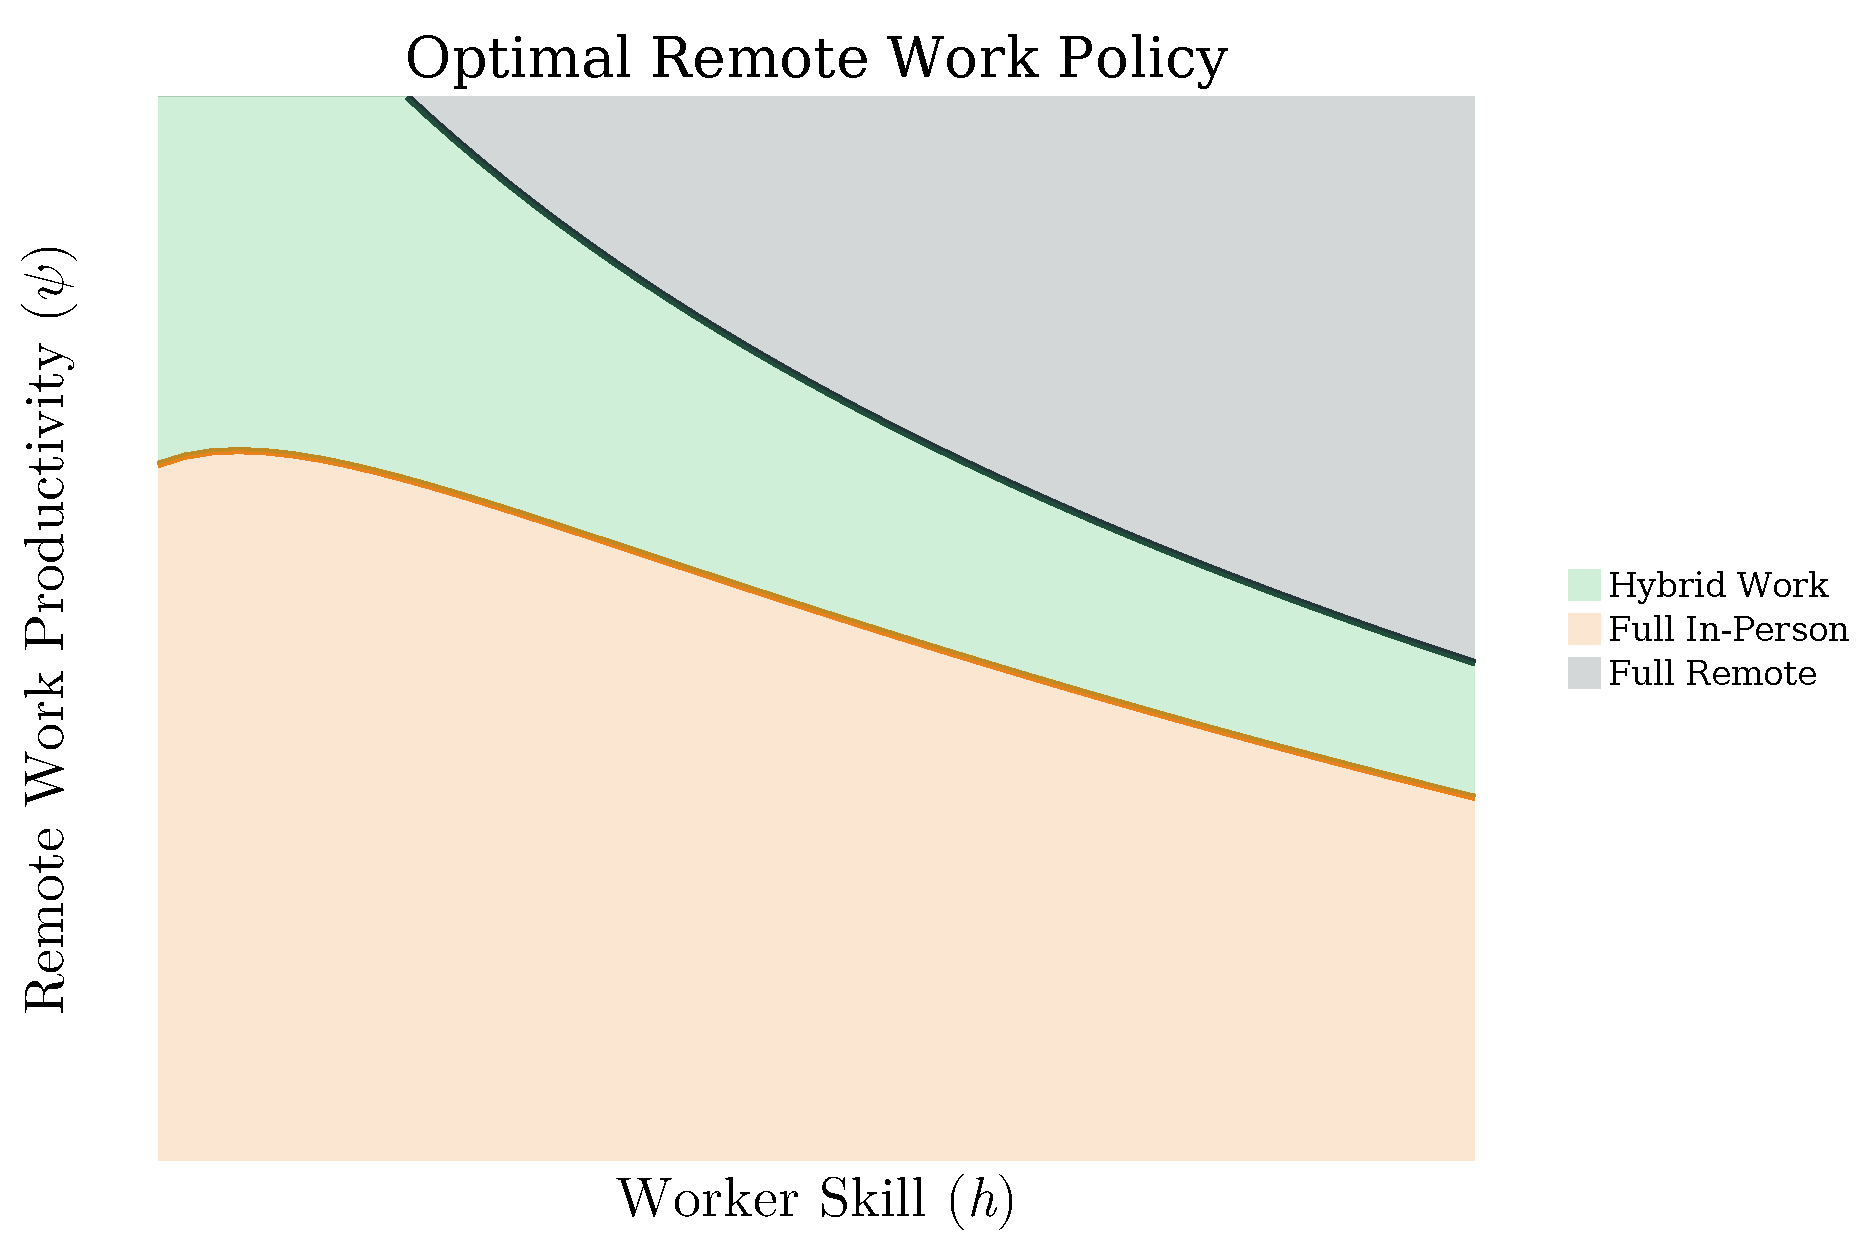
\includegraphics[width=.9\linewidth]{/Users/mitchv34/Work/WFH/figures/model_figures/remote_work_policy.pdf}
    
\end{figure}
    
\end{frame}


\begin{frame}{Value Functions}

    \begin{itemize}
        \item Firms:
        \begin{itemize}
            \item Value of posting:
                \begin{equation*}
                    \underbrace{V(h, x)}_{=0\text{ by free entry}} = - \kappa + q(\theta(h,x))\int J(\psi, h, x) dF(\psi)
                \end{equation*}
            \item Value of an ongoing match:
            \begin{equation*}
                    J(\psi, h, x) = Y(\alpha^*(\psi, h)\mid \psi, h) - w(x, \alpha^*(\psi, h)) + \beta (1 - \delta) J(\psi, h, x)
                \end{equation*}
        \end{itemize}
        \item Workers:
        \begin{itemize}
            \item Value of unemployed worker:
            \begin{equation*}
 U(h) = b + \max_{x}\left\{ p(\theta(h,x))\int W(\psi, h, x) dF(\psi) + (1 - p(\theta(h,x)))U(h)\right\}
            \end{equation*}
            \item Value of employed worker:
            \begin{equation*}
 W(\psi, h, x) = x + \beta \left[ (1 - \delta) W(\psi, h, x) + \delta U(h) \right]
            \end{equation*}
        \end{itemize}
    \end{itemize}
    
\end{frame}

\begin{frame}{Better Jobs are Harder to Find (but better workers find them)}
    \begin{figure}
        \centering
        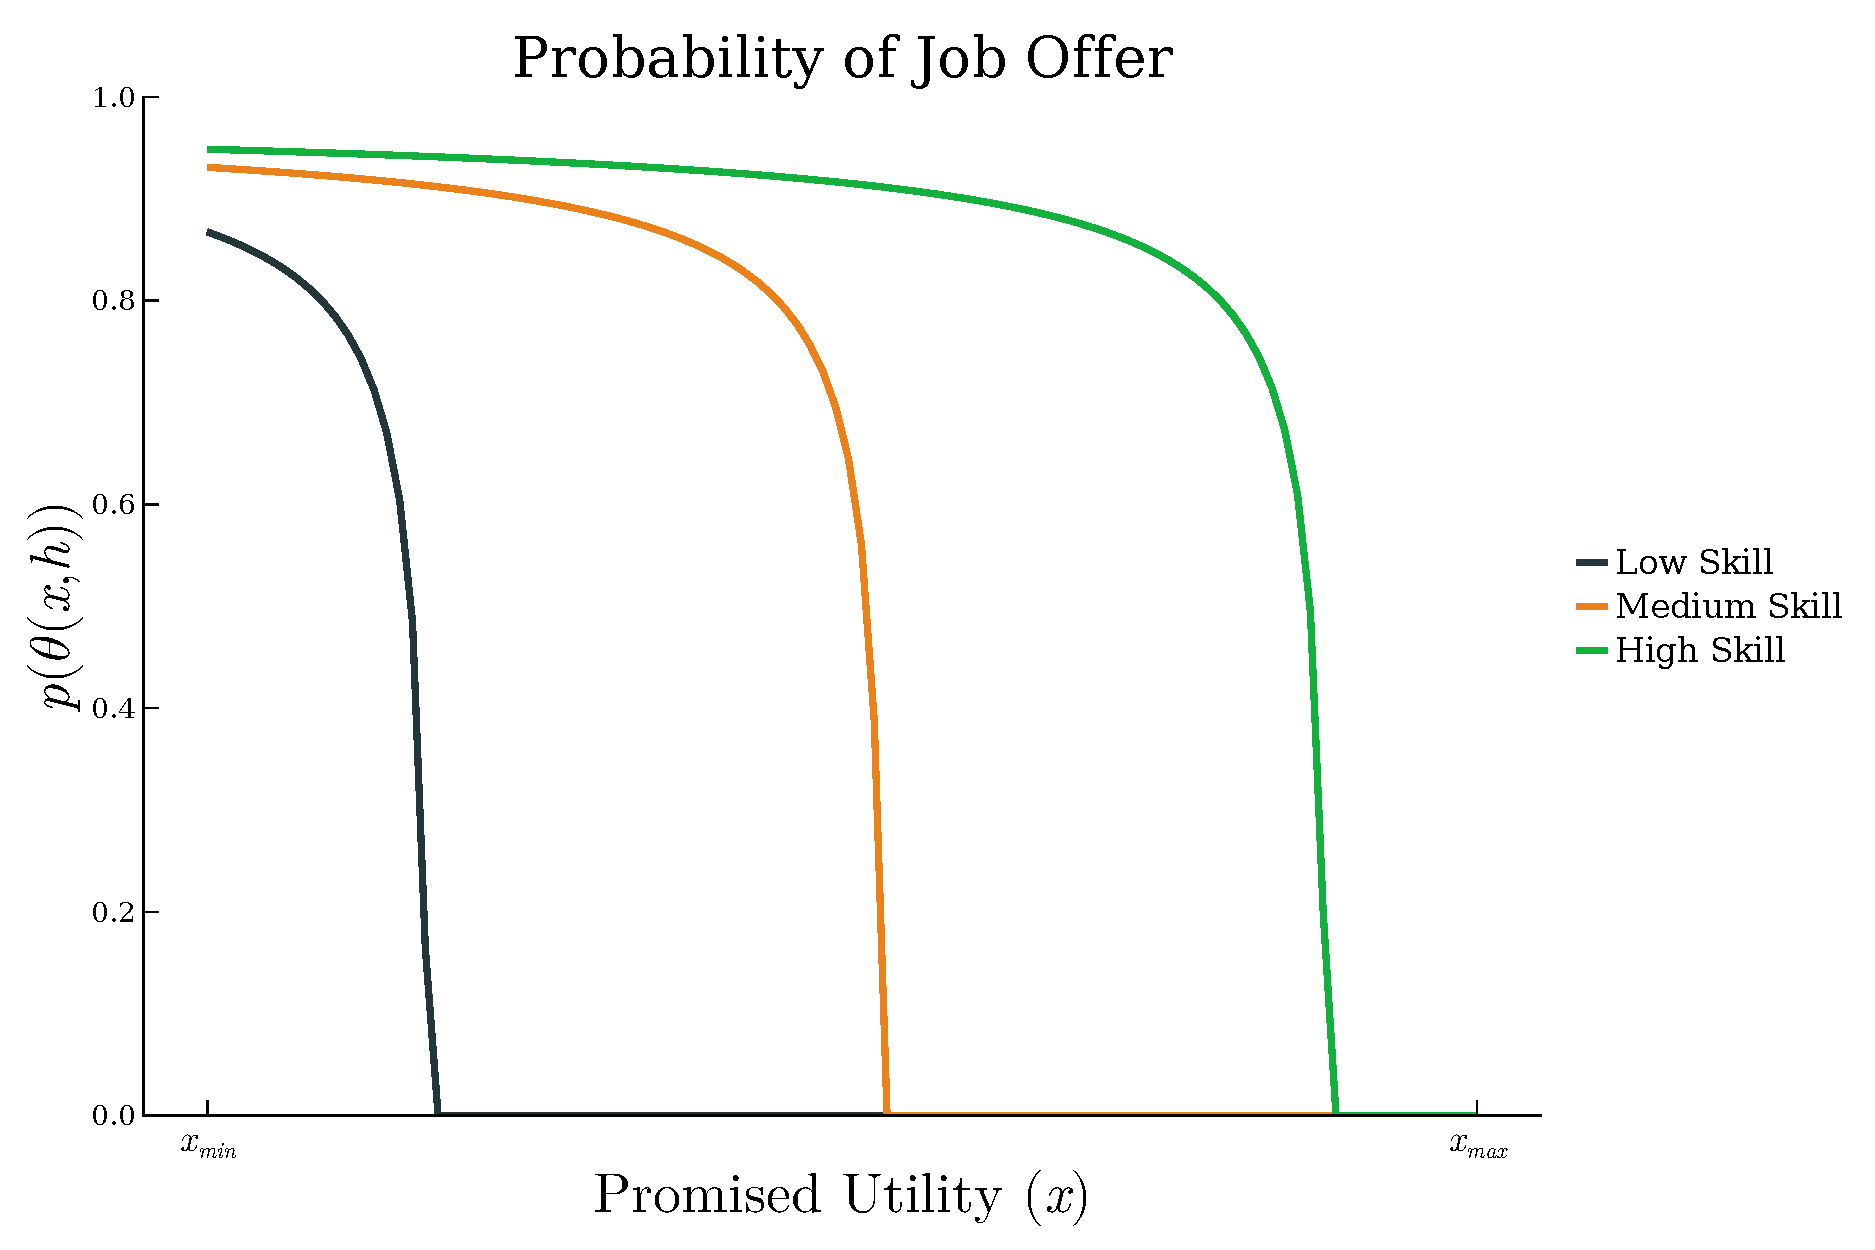
\includegraphics[width=.85\linewidth]{/Users/mitchv34/Work/WFH/figures/model_figures/job_finding_prob.pdf}
    \end{figure}
\end{frame}

\begin{frame}{Higher Skill Workers search for Better Jobs}
    \begin{figure}
        \centering
        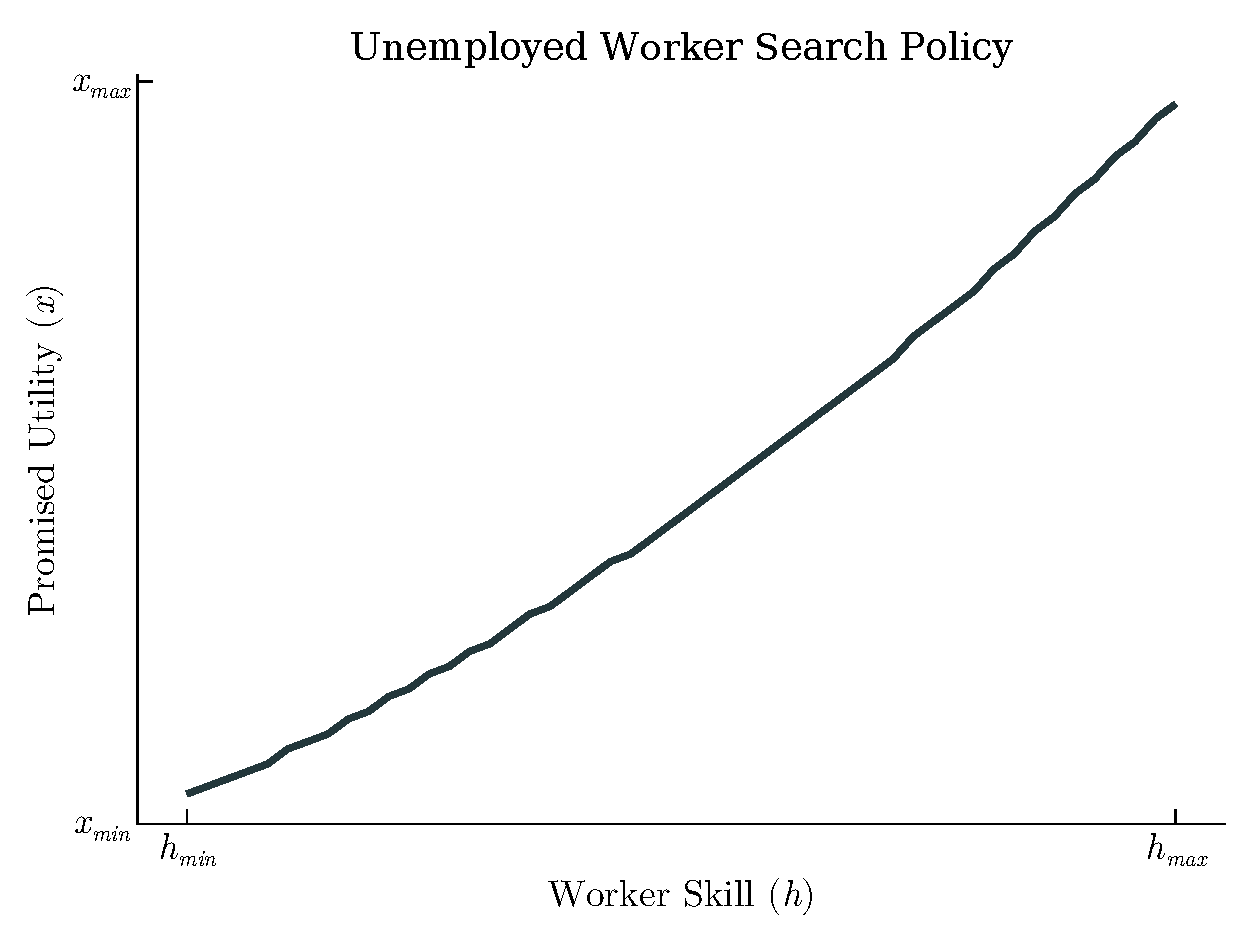
\includegraphics[width=.8\linewidth]{/Users/mitchv34/Work/WFH/figures/model_figures/worker_search_policy.pdf}
    \end{figure}
\end{frame}

\begin{frame}{Higher-Skilled Workers Earn More and Access More Remote Opportunities}
    \begin{figure}
        \centering
        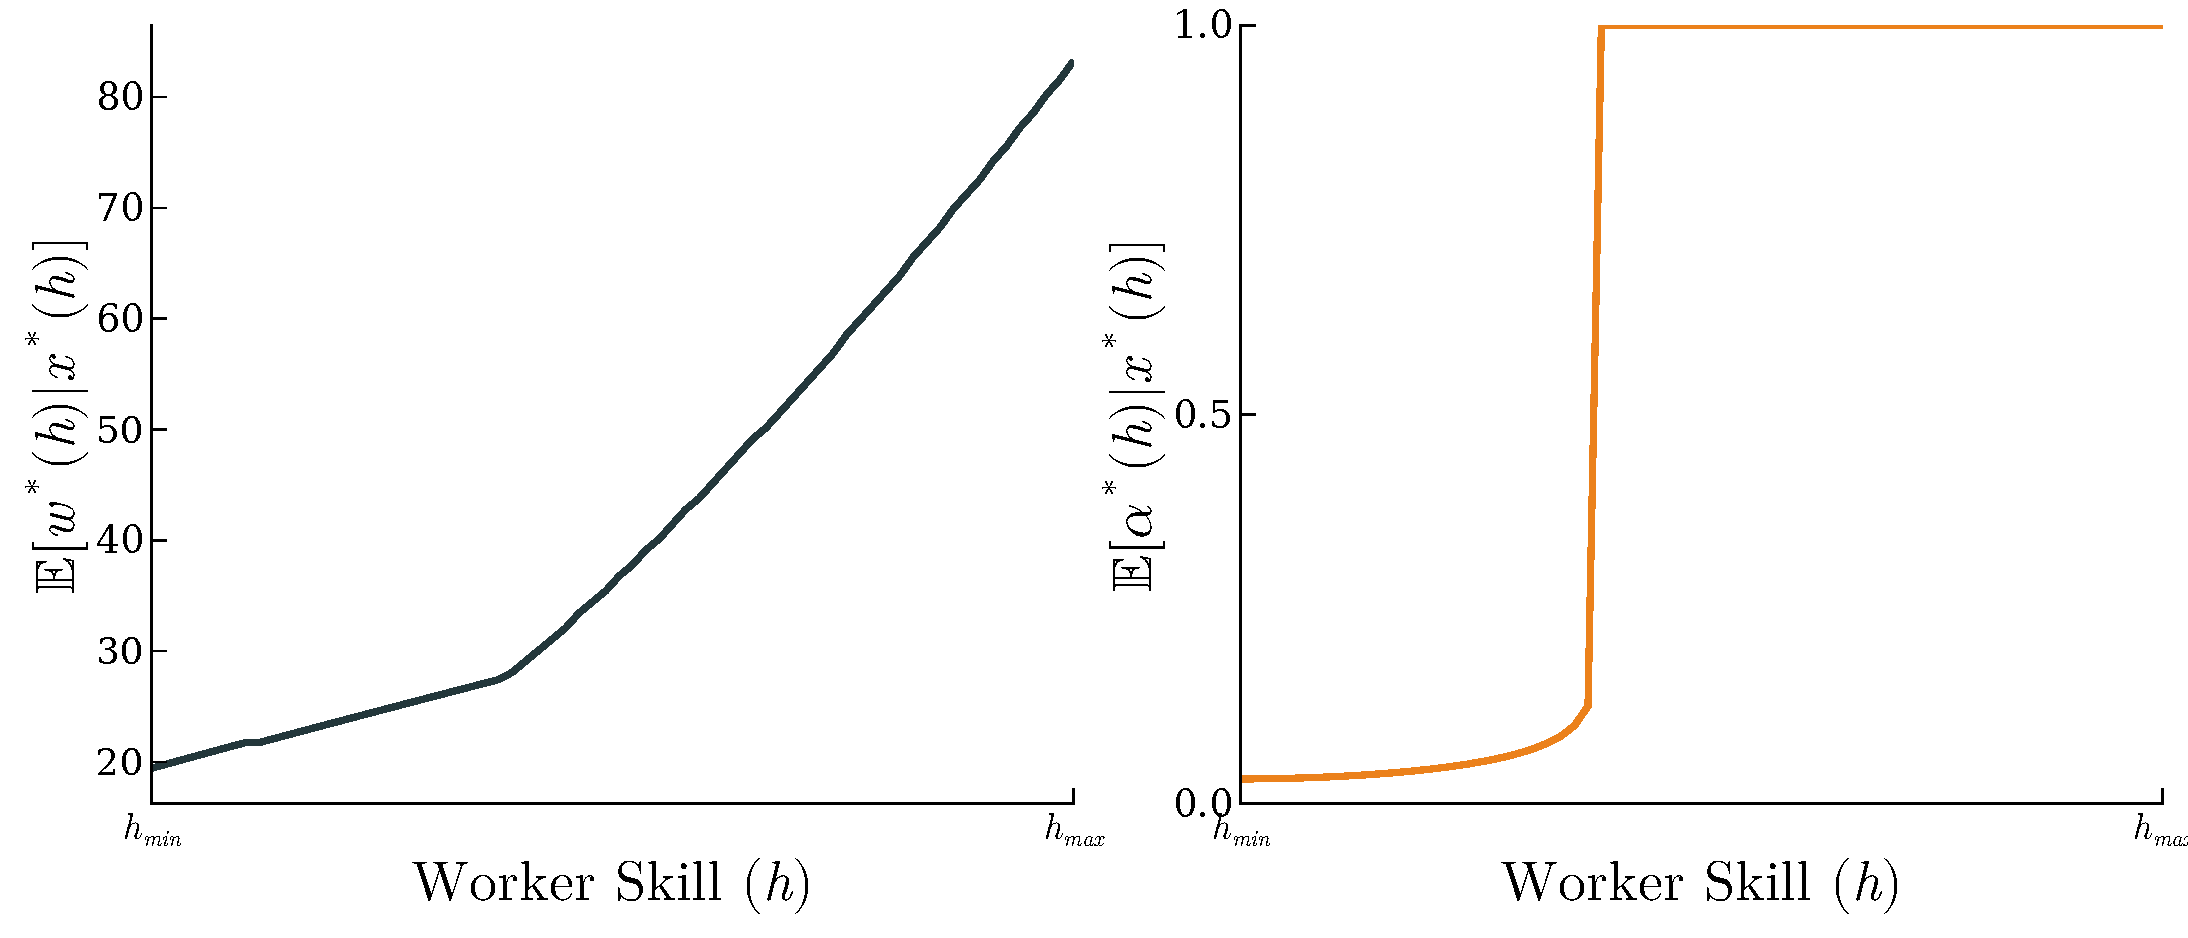
\includegraphics[width=1\linewidth]{/Users/mitchv34/Work/WFH/figures/model_figures/wage_and_remote.pdf}
    \end{figure}
\end{frame}

\section{Calibration}
% --- Slide: Calibration Overview ---
\begin{frame}[label=calibration_overview]{Calibration Overview}
    \begin{itemize}
        \item \textbf{Worker Skill Distribution}:
        \begin{itemize}
            \item Skill index at the occupation level constructed from \textit{Abilities} and \textit{Skills} datasets from ONET.\hyperlink{appendix_worker_skill}{\beamergotobutton{details}}
        \end{itemize}

        \item \textbf{Remote Work Efficiency Distribution}$(F(\psi))$:
        \begin{itemize}
            \item No productivity data at the occupation level.
            \item Labor productivity at the 3-digit industry level from BLS.
            \item Combined with the teleworkability index estimated at the occupation level with the occupation composition of each industry, obtain the remote work feasibility at the industry level.
            \item Use the observed fraction of remote workers in each industry (ACS).
            \item Regress productivity data on remote work indicators to estimate $\psi$ as a function of observables. \hyperlink{appendix_calibration_psi_details}{\beamergotobutton{details}}
            \item Use a kernel density estimator to calibrate the distribution of teleworkability (\(\psi\)).
        \end{itemize}
        
    \end{itemize}
\end{frame}


\begin{frame}{Calibrated Parameters and Density Function}
    \begin{columns}
        % First column: Table of estimated parameters
        \column{0.4\textwidth}
        \centering
        \begin{tabular}{lc}
            \toprule
 Parameter & Estimate \\
            \midrule
            $A$ & 25.55 \\
            $\psi_0$ & 1.46 \\
            $\phi$ & 2.66 \\
            \bottomrule
        \end{tabular}
        \hyperlink{appendix_calibration_psi_details}{\beamergotobutton{details}}
        % Second column: Density plot
        
        \column{0.6\textwidth}
        \centering
        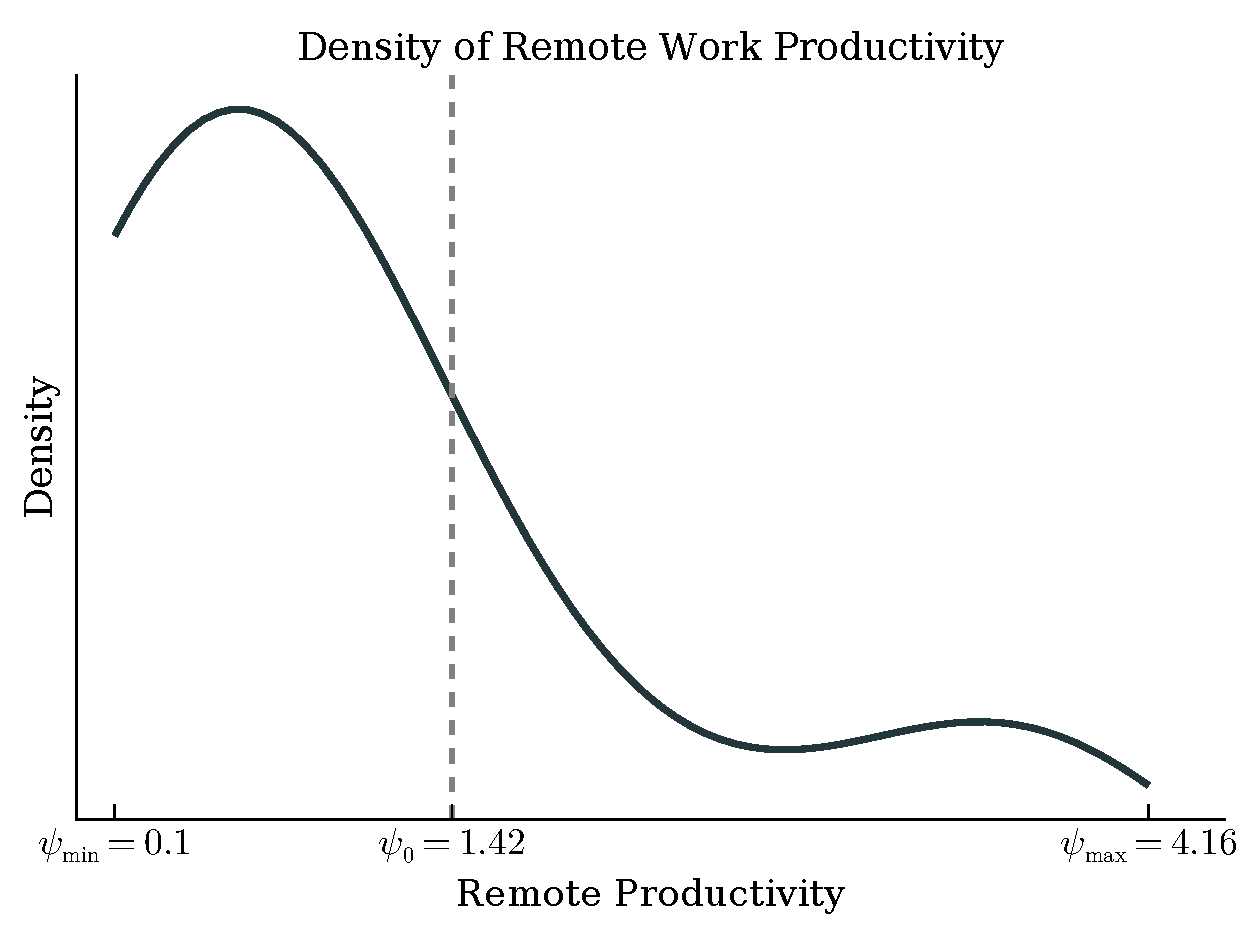
\includegraphics[width=\textwidth]{/Users/mitchv34/Work/WFH/figures/model_figures/productivity_density.pdf}
    \end{columns}
\end{frame}

\begin{frame}{Future Work}
        
    \begin{itemize}
        \item Incorporate additional sources of heterogeneity, firm productivity, and worker preferences.
        \item Test alternative functional forms for productivity and utility in the theoretical model.
        \item Examine how the overall technological environment and digital infrastructure influence remote work feasibility and wage differentials.
        \item Explore dynamic aspects such as on-the-job search and career mobility in remote work settings.
        \item Evaluate counterfactual scenarios—such as a complete shutdown of remote work—to measure their impact on wage differentials.
    \end{itemize} 

\end{frame}

% Appendix for backup slides
\appendix

\begin{frame}[plain]
  \Huge \centering
 Appendix
  \label{appendixstart} % So we can jump here
\end{frame}

\begin{frame}[label=appendix_remote_index_details]{Occupation Remote Index: Details}
 \begin{itemize}
    \item \textbf{Data:} Occupation-level features (tasks, skill requirements, etc.)
    \item \textbf{Models:} SVC (RBF) for classification, SVR (RBF) for teleworkability level.
    \item \textbf{Hyperparameters:} (tuned via cross-validation)
    \item \textbf{Validation:} Boostrap validation (1000 samples) per parameter set.
  \end{itemize}

  \hyperlink{empiric_remote_index1}{\beamergotobutton{Back}}
\end{frame}


\begin{frame}[label=appendix_remote_index_performance_feature_importance_classifier]{Occupation Remote Index: Performance}
    % Figure of feature importance for regressor
    \begin{figure}
        \centering
        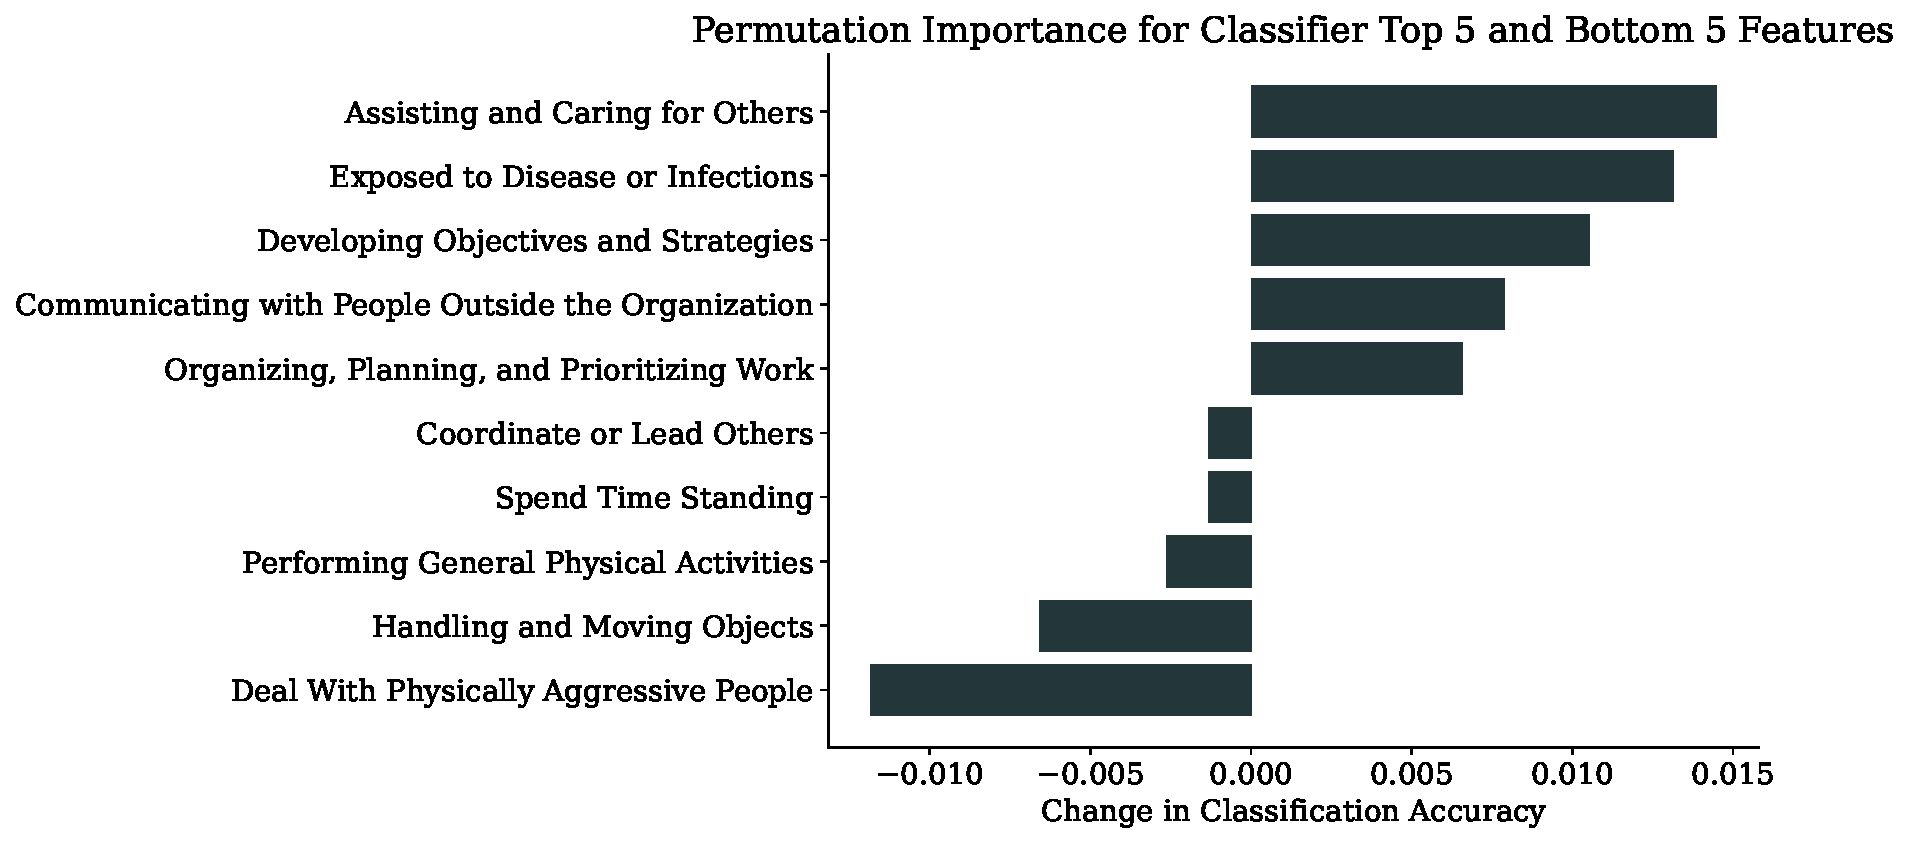
\includegraphics[width=1\textwidth]{/Users/mitchv34/Work/WFH/figures/telework_index_estimation/permutation_importance_classifier.pdf}
        \caption{Feature importance for classifier stage}
    \end{figure}

    \hyperlink{empiric_remote_index1}{\beamergotobutton{back}}
\end{frame}

\begin{frame}[label=appendix_remote_index_performance_feature_importance_regressor]{Occupation Remote Index: Performance}
    % Figure of feature importance for regressor

    \begin{figure}
        \centering
        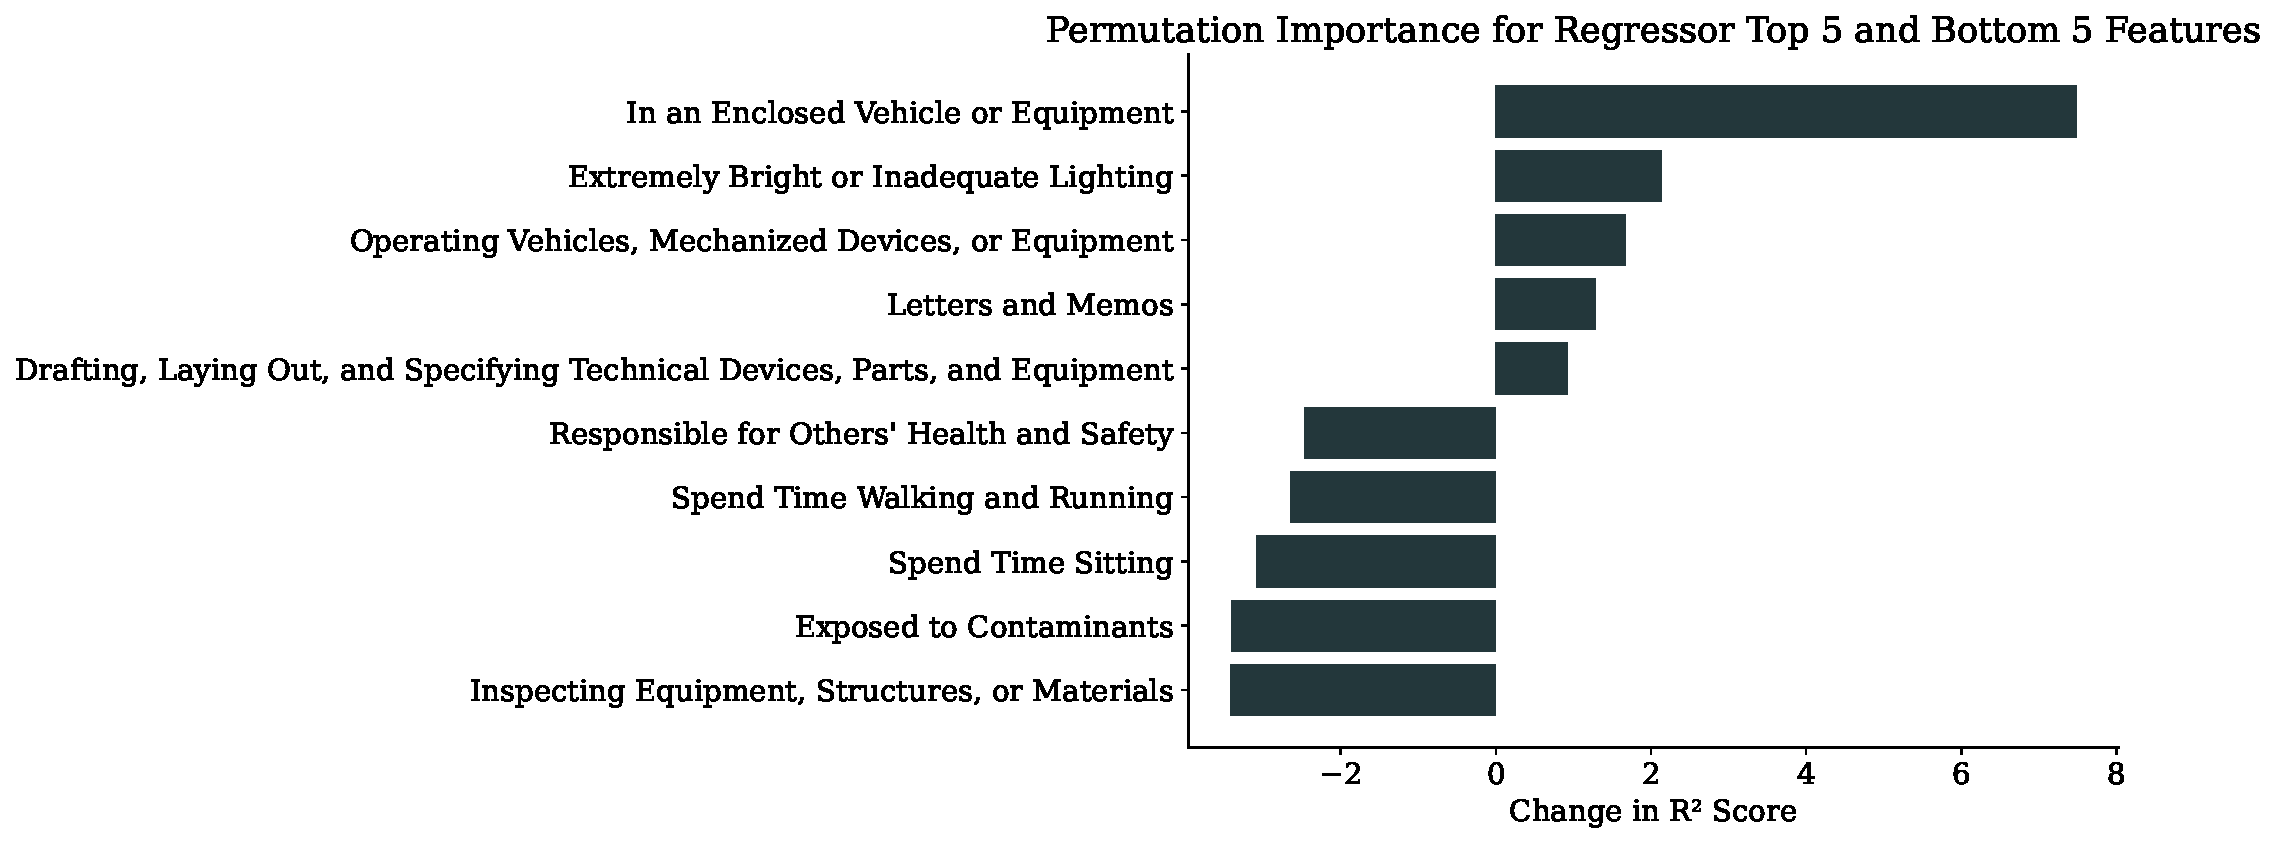
\includegraphics[width=1\textwidth]{/Users/mitchv34/Work/WFH/figures/telework_index_estimation/permutation_importance_regressor.pdf}
        \caption{Feature importance for regressor stage}
    \end{figure}

    \hyperlink{empiric_remote_index1}{\beamergotobutton{back}}
\end{frame}


\begin{frame}[label=appendix_calibration_psi_details]{Calibration of Remote Work Efficiency Distribution}
    
    \begin{itemize}

        \item Consider the production function:
        $$Y(\alpha, h, \psi) = A h ((1-\alpha)  + \alpha (\psi - \psi_0 + \phi \log(h))$$
    
        \item We make the following assumption:
        $$\psi_i = \psi_1 \text{Tele}_i$$
        \item This implies the following specification:
        $$
 Y_{it} = \beta_0 + \beta_1 h_{i} + \beta_2 \alpha_{it} h_{i} + \beta_3 \text{Tele}_i \alpha_{it} + \beta_4 h_{i} \log(h_i)
        $$
        \item This identifies the coefficients:
        $$A = \beta_1, \quad \psi_0 = \frac{\beta_2+1}{A}, \quad \psi_1 =\frac{\beta_3}{A}, \quad \phi = \frac{\beta_4}{A}$$
    \end{itemize}
    \hyperlink{calibration_overview}{\beamergotobutton{Back}}
\end{frame}

\begin{frame}{Calibration of Remote Work Efficiency Distribution: Results}
    $$
    Y_{it} = \beta_0 + \beta_1 h_{i} + \beta_2 \alpha_{it} h_{i} + \beta_3 \text{Tele}_i \alpha_{it} + \beta_4 h_{i} \log(h_i)
    $$
    \begin{table}
        %     \caption{}
        %     \label{}
        \begin{center}
            \footnotesize
        \begin{tabular}{ll}
        \hline
        \hline
                         & $Y$       \\
        \hline
        $\beta_0$        & 16.739\sym{***}   \\
                         & (6.151)     \\
        $\beta_1$            & 25.708\sym{***}   \\
                         & (4.345)     \\
        $\beta_2$      & -37.564\sym{**}   \\
                         & (17.131)    \\
        $\beta_3$ & 315.199\sym{***}  \\
                         & (73.476)    \\
        $\beta_4$ & 64.152\sym{***}   \\
                         & (20.580)    \\
        \hline
        N                & 418         \\
        $R^2$          & 0.263       \\
        \hline
        \hline
        \end{tabular}
        \end{center}
        \end{table}
\end{frame}


\begin{frame}[label = wfhyears_appendix]{WFH premium over years}
\small

\begin{table}[htbp]\centering
\footnotesize
\begin{tabular}{lc}
\toprule
\hline
Dependent variable & Log of real hourly wage \\
\hline
WFH (1 if works from home)       & 0.0781***  (0.005)  \\
WFH\#2014 & 0.0099 (0.0074)  \\
WFH\#2015 & 0.0136* (0.0072)  \\
WFH\#2016 & 0.0134* (0.0069)  \\
WFH\#2017 & 0.0160**  (0.0069)  \\
WFH\#2018 & 0.0178*** (0.0065)  \\
WFH\#2019 & 0.00737  (0.0065)  \\
WFH\#2020 & 0.0243***  (0.0058)  \\
WFH\#2021 & 0.0286*** (0.0056)  \\
WFH\#2022 & 0.0209*** (0.0056)  \\
%Constant                & 1.663***  (0.0029) \\
\hline 
Observations            & 8,410,229 \\
R-squared               & 0.438     \\
\hline 
\bottomrule
\multicolumn{2}{l}{\footnotesize{Fixed effects: Age and age squared,
education controls,
race controls, year FE,
place of residence FE,}}\\
\multicolumn{2}{l}{\footnotesize{industry FE, 
occupation FE. Robust standard errors are in parentheses.}}\\
%\multicolumn{2}{l}{\footnotesize{ Robust standard errors in parentheses.}}\\
%\multicolumn{2}{l}{\footnotesize{*** p<0.01, ** p<0.05, * p<0.1}} 
\end{tabular}
\end{table}
\hyperlink{wfhyears_main}{\beamerskipbutton{Back}}  

\end{frame}


\begin{frame}[label = sfact_1_wage]{Stylized Fact I: Remote Work Correlates with Higher Wages}
    \begin{table}[htbp]
        \centering
        \footnotesize
        \caption{Wage regressed on Teleworkability index and remote work indicator.}
        \begin{tabular}{l c c c c c >{\columncolor{myorange!20}}c}
        \hline \hline  
                            &\multicolumn{1}{c}{(1)}         &\multicolumn{1}{c}{(2)}         &\multicolumn{1}{c}{(3)}         &\multicolumn{1}{c}{(4)}         &\multicolumn{1}{c}{(5)}         &\multicolumn{1}{c}{(6)}         \\
        \hline
 Teleworkability Index          & 33.58\sym{***}& 27.68\sym{***}& 20.89\sym{***}& 19.70\sym{***}& 15.36\sym{***}& 14.90\sym{***}\\
            & (0.0522)         & (0.0580)         & (0.115)         & (0.115)         & (0.0569)         & (0.0570)         \\
 WFH Indicator              &                     &                     &                     & 6.365\sym{***}&                     & 3.203\sym{***}\\
        &                     &                     &                     & (0.0506)         &                     & (0.0487)         \\
        \hline
 FE: Year \& Location            &  $\checkmark$  &  $\checkmark$  &  $\checkmark$  &  $\checkmark$  & $\checkmark$  &   $\checkmark$  \\
 FE: Industry                    &                &  $\checkmark$  &               &  $\checkmark$  &  $\checkmark$  &  $\checkmark$  \\
 AgeCat  $\times$ Educ                &                &               &               &               &  $\checkmark$    &  $\checkmark$  \\
        \hline
 N                   & 9708029         & 9708029         & 9708029         & 9708029         & 9708028         & 9708028         \\
        $R^2$                  & 0.141         & 0.186         & 0.227         & 0.230         & 0.292         & 0.293         \\
        \hline\hline
\multicolumn{7}{l}{\footnotesize Worker level data. All regressions include demographic controls: age, race, education, others.}\\
\multicolumn{7}{l}{\footnotesize Standard errors in parentheses: \sym{*} \(p<0.1\), \sym{**} \(p<0.05\), \sym{***} \(p<0.001\).}\\
        \end{tabular}
    \end{table}
    \hyperlink{sfact_1_logwage}{\beamerskipbutton{Wage regression}}
\end{frame}

\begin{frame}[label = sfact_2_wage]{Stylized Fact II: Within Occupations Remote Workers Earn More}

\begin{table}[htbp]
    \centering
    \footnotesize
    \caption{Wage regressed on remote work indicator and controls. }
    \begin{tabular}{l c c c c >{\columncolor{myorange!20}}c}
    \hline\hline  
                    & \multicolumn{1}{c}{(1)}         & \multicolumn{1}{c}{(2)}         & \multicolumn{1}{c}{(3)}         & \multicolumn{1}{c}{(4)}         & \multicolumn{1}{c}{(5)}         \\
\hline
WFH Indicator              & 12.44\sym{***}& 7.702\sym{***}& 5.834\sym{***}& 5.031\sym{***}& 3.603\sym{***}\\
& (0.0530)         & (0.0525)         & (0.0494)         & (0.0493)         & (0.0471)         \\
\hline
FE: Year \& Location            &  $\checkmark$  &  $\checkmark$  &  $\checkmark$  &  $\checkmark$  &  $\checkmark$  \\
FE: Industry                    &                &  $\checkmark$  &               &  $\checkmark$  &  $\checkmark$  \\
FE: Occupation                  &                &               &  $\checkmark$  &  $\checkmark$  &  $\checkmark$  \\
FE: Class of Worker             &                &               &               &  $\checkmark$  &  $\checkmark$  \\
AgeCat  $\times$ Educ                &                &               &               &               &  $\checkmark$  \\
\hline
N                   & 9712293         & 9712293         & 9712293         & 9712293         & 9712292         \\
$R^2$               & 0.0711         & 0.153         & 0.289         & 0.307         & 0.364         \\
\hline\hline
\multicolumn{6}{l}{\footnotesize Worker level data. All regressions include demographic controls: age, race, education, others.}\\
\multicolumn{6}{l}{\footnotesize Standard errors in parentheses: \sym{*} \(p<0.1\), \sym{**} \(p<0.05\), \sym{***} \(p<0.001\).}\\
    \end{tabular}
\end{table}
\hyperlink{sfact_2_logwage}{\beamerskipbutton{Wage regression}}
\end{frame}


\begin{frame}[label=appendix_worker_skill]{Worker's Skill Distribution}
    \begin{columns}
        \column{0.3\textwidth}
        \begin{itemize}\footnotesize
            \item The skill distribution is constructed from ONET data.
            \item Simple average of Skills and Abilities weighted by importance to the occupation.
            \item We fit a Normal distribution to the skill index.
            \begin{itemize}\footnotesize
                \item \textbf{Mean:} 0.41
                \item \textbf{Standard Deviation:} 0.17
            \end{itemize}
        \end{itemize}
        \column{0.7\textwidth}
        \begin{figure}
            \centering
            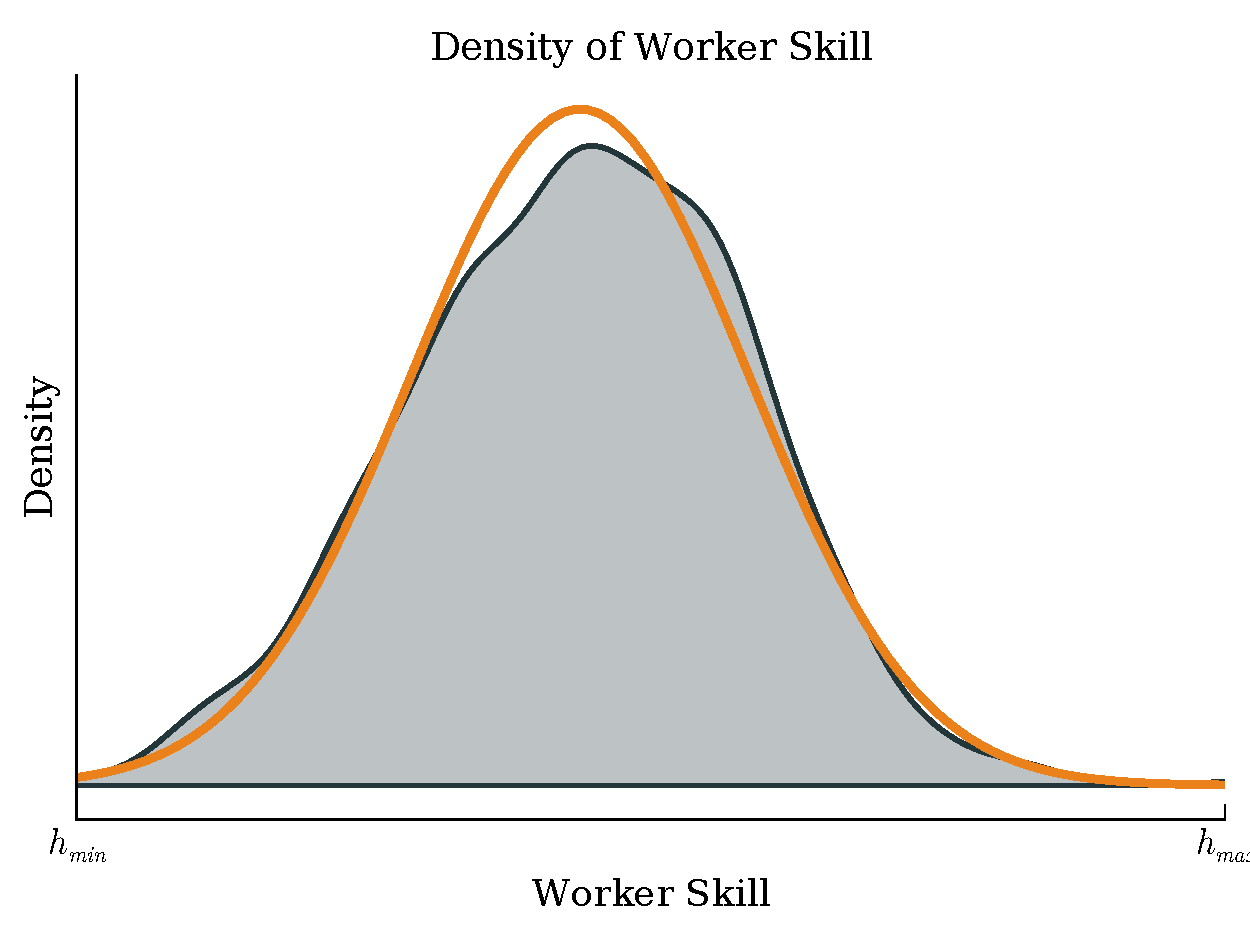
\includegraphics[width=\linewidth]{/Users/mitchv34/Work/WFH/figures/model_figures/skill_distribution.pdf}
        \end{figure}
    \end{columns}
    \hyperlink{calibration_overview}{\beamergotobutton{Back}}
\end{frame}

\end{document}